\subsection{Pojęcia i zasady}

\subsubsection{Wstęp}
Ta podsekcja dokumentuje Lupus w formie wyjaśniania zdefiniowanych na jego potrzeby pojęć, konceptów i zasad. Są one punktem wyjścia do dokładniejszych specyfikacji i zarazem zrozumienia architektury systemu. Sekcja ta zawiera wiele linków do definicji znajdujących się w załączniku i nie wszystkie pojęcia tłumaczone są w tej sekcji.

\subsubsection{Problem zarządzania}

W rzeczywistym świecie często napotkamy sytuacje, w których byłoby dobrze, gdyby praca jakiegoś systemu mogła być stale regulowana. Na przykład:

\begin{itemize}
    \item chcielibyśmy, aby samochody miały funkcję regulującą pracę silnika w celu utrzymania stałej prędkości,
    \item przydałoby się, gdyby lodówka mogła utrzymywać chłodną, ale nie ujemną temperaturę, niezależnie od tego, jak często otwierane są drzwi lub jaka jest temperatura na zewnątrz w danym dniu,
    \item byłoby korzystne, gdyby serwer w chmurze mógł zagwarantować, że aplikacja z wystarczającymi zasobami do pokrycia potrzeb użytkowników będzie uruchomiona i działała.
\end{itemize}

Problemy wymienione powyżej można traktować jako \textbf{problemy zarządzania} (ang. \textit{management problem}). Nazwa bierze się stąd, że nie ma żadnych technicznych ograniczeń uniemożliwiających osiągnięcie tych celów. Wszystkie wymienione systemy są odpowiednio wyposażone np. możemy dodać więcej paliwa do silnika lub dostarczyć więcej mocy do sprężarki w lodówce. Problem leży w faktycznym wykonaniu tych czynności w odpowiednich momentach np. dodanie więcej paliwa, gdy auto zwalnia lub dostarczenie większej mocy gdy temperatura w lodówce wzrasta. Dlatego jest to problem czystego zarządzania.

Za to system, którym chcemy zarządzać nazywamy \textbf{zarządzanym systemem} (ang. \textit{managed system}). 

\subsubsection{System kontroli}

\textbf{System kontroli} (ang. \textit{Control System\footnote{innym tłumaczeniem na polski jest "regulator"}} to system, który reguluje pracą \textbf{zarządzanego systemu}. Na przykład:
\begin{itemize}
    \item tempomat, który reguluje pracą silnika w celu utrzymania stałej prędkości,
    \item lodówka, która reguluje pracą sprężarki w celu utrzymania stałej, chłodnej temperatury
    \item Kubernetes, który reguluje liczbę działających Podów, aby utrzymać pożądaną dostępności aplikacji
\end{itemize}

Innymi słowy mówiąc \textbf{System kontroli} rozwiązuje \textbf{Problem Zarządzania}.

\subsubsection{Pętla sterowania}

Ogólną architekturą \textbf{Systemów Kontroli} używaną do rozwiązywania \textbf{Problemów Zarządzania} jest \textbf{Pętla Sterowania}.

Pętle sterowania są klasyfikowane w zależności od tego, czy wykorzystują mechanizmy sprzężenia zwrotnego (ang. \textit{feedback mechanism}):
- \textbf{Otwarte Pętle Sterowania}: Akcja Sterująca (ang. \textit{Control Action}) (czyli wejście do \textbf{Systemu Zarządzanego}) jest niezależne od wyjścia \textbf{Systemu Zarządzanego}.
- \textbf{Zamknięte Pętle Sterowania}: Wyjście \textbf{Systemu Zarządzanego} jest sprzężane do wejścia \textbf{Systemu Kontroli} i wpływa na Akcję Sterującą. 

W Lupus bierzemy pod uwagę wyłącznie zamknięte pętle sterowania.

\subsubsection{Zamknięta Pętla Sterowania}

Jest to punk wyjściowy (startowy) dla naszej architektury referencyjnej (rys \ref{fig:33-arch}).

\begin{figure}[!h]
    \centering 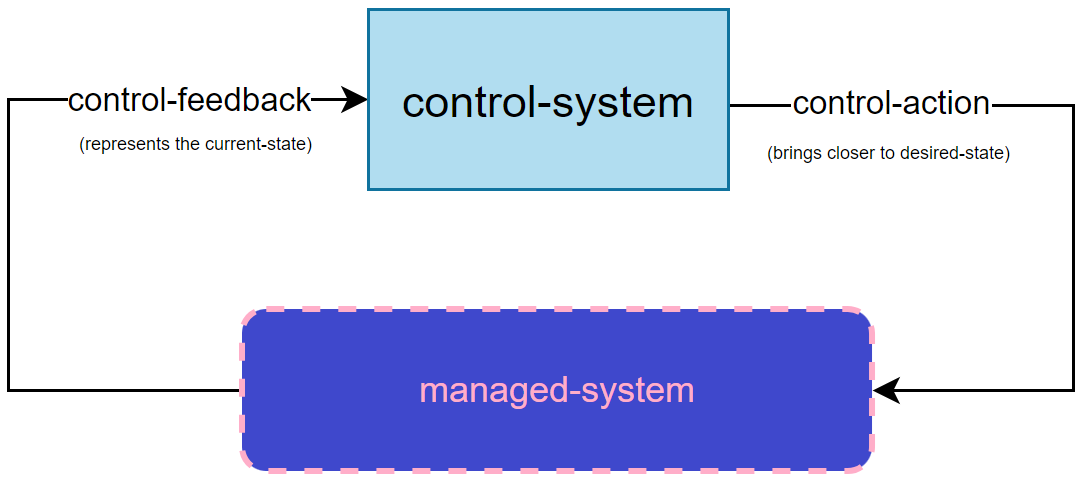
\includegraphics[width=1\linewidth]{33-arch.png}
    \caption{Architektura referencyjna dla Lupus}\label{fig:33-arch}
\end{figure}

Architektura (rys. \ref{fig:33-arch}) należy czytać mając na uwadze następujące definicje:

\begin{itemize}
    \item \textbf{System Sterowania (ang. \textit{Control System})} - system, który rozwiązuje \textbf{Problem Zarzadzania} \textbf{Zarządzanego Systemu} za pomocą \textbf{Zamkniętej Pętli Sterowania}. W każdej iteracji \textbf{System Sterowania} analizuje \textbf{Sprzeżenie Zwrotne} (ang. \textit{Control Feedback}) i \textit{wnioskuje} \textbf{Akcje Sterującą}.
    \item \textbf{Zamknięta Pętla Sterowania} - nieskończona pętla, która reguluje stan \textbf{Zarządzanego Systemu}, iteracyjnie zbliżając jego \textbf{Aktualny Stan} do \textbf{Stanu Pożądanego}. 
    \item \textbf{Akcja Sterująca (ang. \textit{Control Action})} - akcja wykonywana na \textbf{Zarządzanym Systemie}, która ma na celu przybliżenie go do \textbf{Stanu Pożądanego}.
    \item \textbf{Sprzeżenie zwrotne} (ang. \textit{Control Feedback}) - reprezentacja \textbf{Aktualnego Stanu} wysyłana z (odbierana od) \textbf{Systemu Zarządzanego}.
\end{itemize}

W powyższej architekturze Lupus pełni rolę \textbf{Systemu Sterowania}.

\subsubsection{Agenci Translacyjni}
Z racji, że każdy system, bez żadnych modyfikacji (\ref{reg:7}) może wejść w rolę \textbf{Zarządzanego Systemu}, potrzebujemy warstwy integracji między \textbf{systemem zarządzanym} a Lupus, podobna do koncepcji "API Broker" w architekturze ENI (rys. \ref{fig:23-eni-arch}). Tak narodziła się koncepcja \textbf{Agentów Translacyjnych} (ang. \textit{Trasnlation Agents}). 

W każdym \textbf{wdrożeniu Lupus}, \textbf{użytkownik} musi stworzyć \textbf{Agentów Translacyjnych}. 

Z punktu wiedzenia komunikacji, każdego \textbf{Agenta Translacyjnego} możemy podzielić na dwie części:
\begin{itemize}
    \item Część komunikująca się z \textbf{Systemem Zarządzanym}. Jest to zewnętrzna względem Lupus i nie podlega żadnej specyfikacji.
    \item Część komunikująca się z Lupus. Musi być zgodne z jednym z interfejsów Lupus. \textbf{Lupin} lub \textbf{Lupout}.
\end{itemize}

Mamy dwóch \textbf{Agentów Sterowania}, jeden do komunikacji przychodzącej (ang. \textit{Ingress}) i jeden do wychodzącej (ang. \textit{Egress}). 

W każdej iteracji pętli zadaniem \text{Agenta Ingress} jest odbieranie/zbieranie \textbf{Sprzężenia Zwrotnego} z \textbf{Systemu Zarządzanego} i translacja go na format zrozumiały przez Lupus za pomocą \textbf{Interfejsu Lupin}. Z kolei zadaniem \textbf{Agenta Egress} jest odbieranie \textbf{final-data}'y i translacja jej na \text{Ackje Sterowania}, która później zostaje wysłana do (lub przeprowadzona na) \text{Systemie Zarządzanym}.

Architektura wraz z wprowadzeniem \textbf{Agentów Translacji} ukaza jest na rysunku \ref{fig:33-arch2}.

\begin{figure}[!h]
    \centering 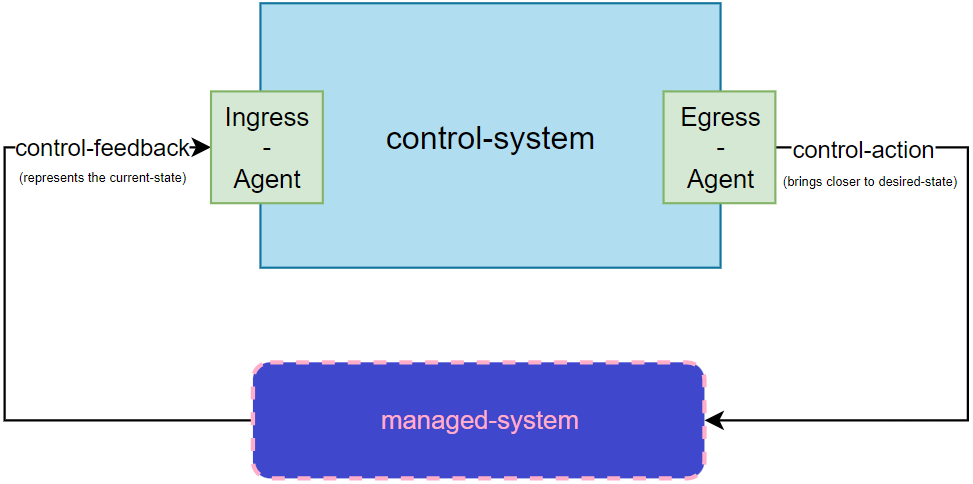
\includegraphics[width=1\linewidth]{33-arch2.png}
    \caption{Architektura referencyjna z agentami translacji}\label{fig:33-arch2}
\end{figure}

Specyfikacja interfejsów \textbf{Lupin} oraz \textbf{Lupout} zawarta jest w załączniku //TODO.

\subsubsection{Workflow pętli}

Kiedy Lupus otrzyma \textbf{Aktualny Stan} poprzez interfejs \textbf{Lupin}, rozpoczyna się \textbf{Workflow Pętli}, które ma na celu dostarczać \textbf{Logikę Pętli} (ang. \textit{Loop Logic}) i składa się z \textbf{Elementów Pętli} (ang. \textit{Loop elements}). 

Elementem pętli może być zarówno:
\begin{itemize}
    \item \text{Element Lupus}, który działa w warstwie sterowania Kubernetes a jego misją jest wykonywać \textit{Workflow Pętli}
    \item referencja do \textbf{Elementu Zewnętrznego}, który działa poza warstwą sterowania Kubernetes a jego misją jest wykonywać \textbf{Część Obliczeniową} \textbf{Logiki Pętli}
\end{itemize}

\textbf{Workflow Pętli} jest wyrażany w \textbf{LupN}, specjalnej notacji do opisywania workflow pętli, której dokładna specyfikacja znajduje się w załączniku //TODO.

Przykładowe \textbf{workflow pętli} pokazano na rysunku \ref{fig:33-workflow}

\begin{figure}[!h]
    \centering 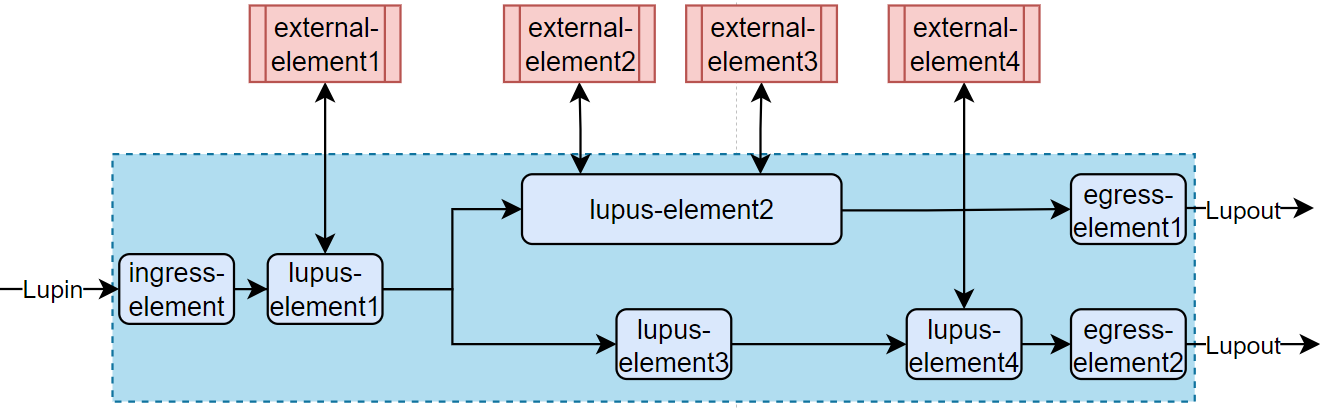
\includegraphics[width=1\linewidth]{33-workflow.png}
    \caption{Przykładowe workflow pętli}\label{fig:33-workflow}
\end{figure}

\begin{itemize}
    \item Niebieskie, zaokrąglone prostokąty reprezentują elementy Lupus,
    \item Czerwone prostokąty oznaczają elementy zewnętrzne.
    \item Niebieski obszar wyznaczony linią przerywaną wskazuje elementy działające w klastrze Kubernetes. Wyróżniono elementy Lupus odpowiedzialne za ingress i egress.
\end{itemize}

\textbf{Elementy Zewnętrzne} to zazwyczaj serwery HTTP (w szczególności serwery Open Policy Agent).

Jak można zauważyć, jeden \textbf{Element Lupus} może komunikować się z zerem, jednym lub wieloma elementami zewnętrznymi (liczba ta może się różnić w każdej iteracji pętli).
